\label{chp:Method}
% 4.1. Overview
\section{Overview of the Proposed System}
..
\cite{Leal-Taixe_2016_CVPR_Workshops}

% 4.2. Data Acquisition
\section{Preprocessing}
\label{sec:preprocessing}

% 4.3. Proposed Methodology
\section{Proposed Methodology}
\label{sec:methodology}
%purpose
In this paper, we propose person identity verification system based on the in-air handwritten Wi-Fi signature signals (which will be called Wi-Fi signature hereafter). 
%function
In order to learn the direction-invariant deep representations for in-air signature, we used the triplet network[] which utilizes ConvNet[] as a feature extractor. Moreover, to achieve a faster loss convergence, we adopt the kernel and the range (KAR) space learning[] for mining the triplet input. 
% figure
\begin{figure*}[!ht]
    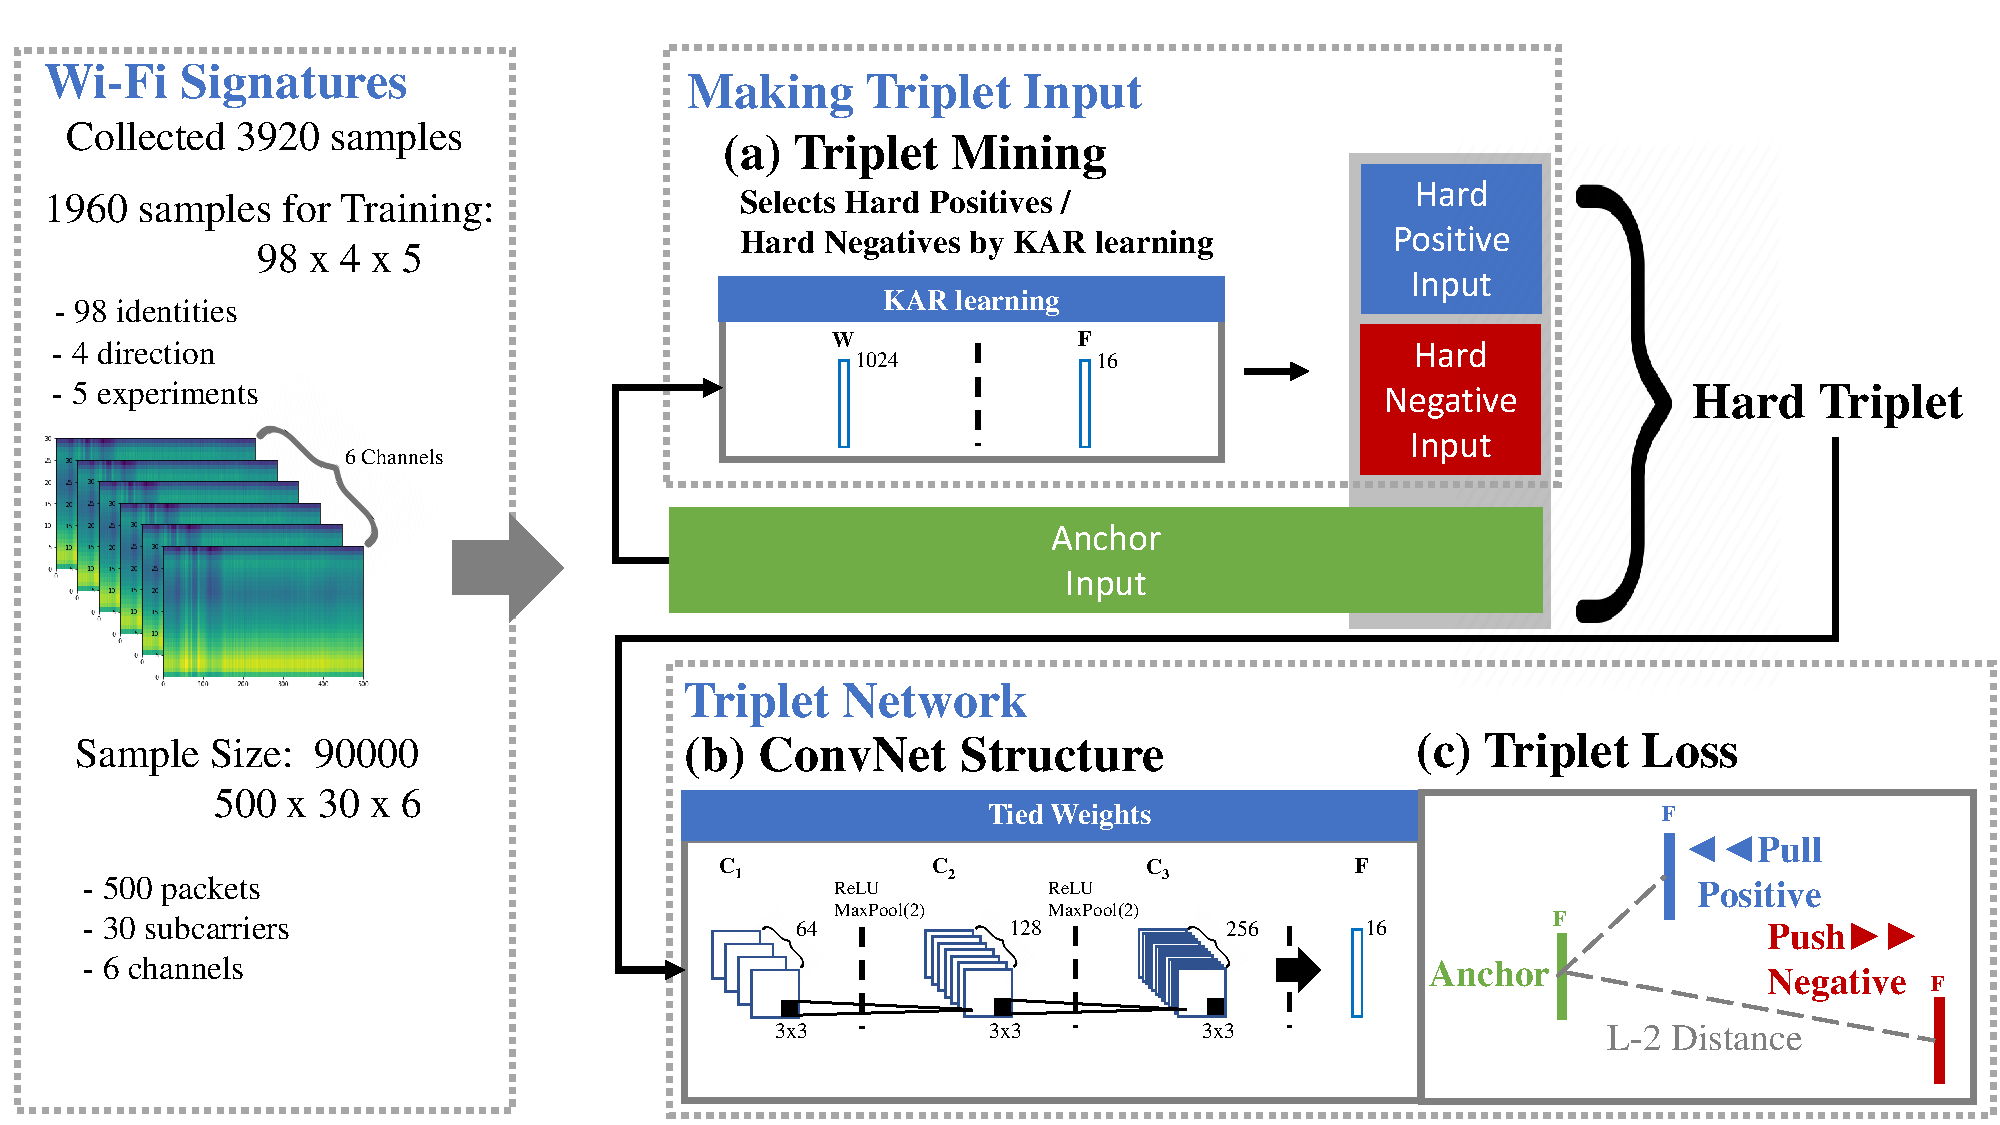
\includegraphics[width=\textwidth]
        {fig_system_overview_v1.pdf}
    \caption{An overview of the proposed methodology.} \label{fig1}
\end{figure*}
Figure~\ref{fig1} shows an overview of the proposed system. 
Essentially, the KAR space projection learning is applied to mine the hard samples from the training dataset for making the triplet input (see item (a) in Fig.~\ref{fig1}). The anchor sample is randomly selected from the training dataset as the reference data. The hard samples refer to which likely to be misclassified by the triplet network for given anchor sample.
Subsequently, the ConvNet structure that forms triplet network (see item (b) in Fig.~\ref{fig1}) is trained based on a triplet loss function based on the distance comparison for network output vector (see item (c) in Fig.~\ref{fig1}).
% following~
In the following subsections, we introduce the triplet network architecture, triplet loss, and triplet mining using KAR space learning in detail.

% 4.4.1. Triplet loss
\subsection{Triplet loss}
% purpose
The purpose of the triplet loss [] is training the ConvNet structure to learn discriminative features that allocates the samples of the same class closer and the samples of the different class far away in the feature space.
% Triplet input
The triplet input is made up of a combination of three samples, anchor sample $x_0$, positive sample $x_+$ and negative sample $x_-$. The anchor sample, which is the reference for the triplet input, is selected from the training data set. For selected anchor sample $x_0$, positive sample is selected from same identity with that of the anchor while negative sample is selected from different identity from that of the anchor.
% function
To make the discriminative feature vectors, we need $dist\{f(x_0),f(x_+)\}$, the distance  between feature vectors of anchor $f(x_0)$ and positive sample $f(x_+)$ is larger than $dist\{f(x_0),f(x_-)\}$, distance between feature vectors of anchor and negative sample  plus preset margin $\alpha$. 
Distance measurement function is shown below:
\begin{equation}
    dist\{f(x_0),f(x_-)\} - dist\{f(x_0),f(x_+)\} \geqq \alpha
    \label{triplet_condition}
\end{equation}
By using $L2$ distance as distance function, triplet loss is calculated as below:
\begin{equation}
    triplet\_loss = \sum_i^N max\left({ \left[ {\left\| {{f(x_0)} - {f(x_+)}} \right\|_2^2} - {\left\| {{f(x_0)} - {f(x_-)}} \right\|_2^2}  + \alpha \right]},0 \right),
    \label{triplet_loss}
\end{equation}
% need to make hard triplets
Note that if $dist\{f(x_0),f(x_-)\}$ is much larger than $dist\{f(x_0),f(x_+)\} + \alpha$, the output of the loss function would be zero. In this case, it may slow down the convergence speed of the training of deep network. However, it is likely to fall into this condition if we randomly select training samples to make a triplet input. For fast loss convergence, we need to mine the triplet input that make the output of our network satisfy the condition~\ref{triplet_condition} to ensure that the output of the loss function is non-zero.

% 4.4.2. Triplet mining
\subsection{Triplet Mining based on the Kernel and the Range space learning}
% purpose
In order to train the network faster, we propose training a sub-network for minining the hard positive and the hard negative sample from the training dataset.

% hard sample
The hard positive sample is the samples which is likely to be misclassified as a negative sample by the triplet network.
In other words, the distance between feature vectors of anchor and hard positive sample is larger than other positive samples.
On the other hand, the hard negative sample is likely to be misclassified as a positive sample since the distance between feature vectors of anchor and this hard negative sample is smaller than other negative samples.
Hard triplet input is made by combining hard positive and hard negative samples for selected anchor samples. By using hard triplet as input to the triplet network, it is easier to satisfy the conditions of~\ref{triplet_condition}. However, we don't know which sample is the hard sample before training the triplet network.

% functions
To make the hard triplet input before tranining the triplet network, we propose training a small sub-network before triplet network.
This small sub-network is made of Multi Layer Perceptron (MLP) and we adopt the Kernel And the Range (KAR) space learning to train the MLP sub-network. As the KAR space learning has no backpropagation and no iterative learning process, we can train this sub-network with the single shot utilizing the entire training dataset $X$. 
Given entire training dataset $X$, the sub-network output is given as: 
\begin{equation}
    KAR\left(\mathbf{X}\right)=\sigma\left(\left[\mathbf{1},\sigma\left(\dots\left[\mathbf{1},\sigma\left(\left[\mathbf{1},\sigma\left(\mathbf{X}\cdot\mathbf{W}_{1}\right)\right]\mathbf{W}_{2}\right)\right]\dots\mathbf{W}_{(n-1)}\right)\right]\mathbf{W}_{n}\right).
\end{equation}
After training the sub-network, we can mine the hard sample by measuring the $L2$ distance between every output vector of the sub-network and output vector of anchor sample.
The sub-network output of a given anchor sample $x_0$ is $KAR(x_0)$, To mine hard-positive sample, select one sample among the sub-network output which distance to anchor feature vector $KAR(x_0)$ is larger than threshold $t_+$. For hard-negative sample, choose one among the sub-network output which distance to anchor feature vector is smaller than threshold $t_-$.
Selected hard-positve and hard-negative sample satisfies this property:
\begin{equation}
    {\left\| {{KAR\left(\mathbf{x}_{0}\right)} - {KAR\left(\mathbf{x}_{+}\right)}} \right\|_2^2} \geq \mathrm{t}_{+}, 
    \label{thres_pos}
\end{equation}
\begin{equation}
    {\left\| {{KAR\left(\mathbf{x}_{0}\right)} - {KAR\left(\mathbf{x}_{-}\right)}} \right\|_2^2} \leq \mathrm{t}_{-},\label{thres_neg}
\end{equation}
If the hardest sample, it is known that the outlier data is likely to be selected and there is a risk of overfishing[].
To avoid this problem, threshold for the hard-positive and the hard-negative samples are empirically chosen as 25 and 75 percentiles of the distance between anchor and sub-network outputs.

% 4.4.3. ConvNet Structures
\subsection{The ConvNet structures}
% Purpose
Since the three-dimensional formats of our input signature signal can be considerd as an image data, we utilized deep ConvNet structure as a feature extractor. This ConvNet structure are made of three layers of ConvNet with triplet loss. Each layers of ConvNet shares their weights. 
% figure
\begin{figure*}[!ht]
    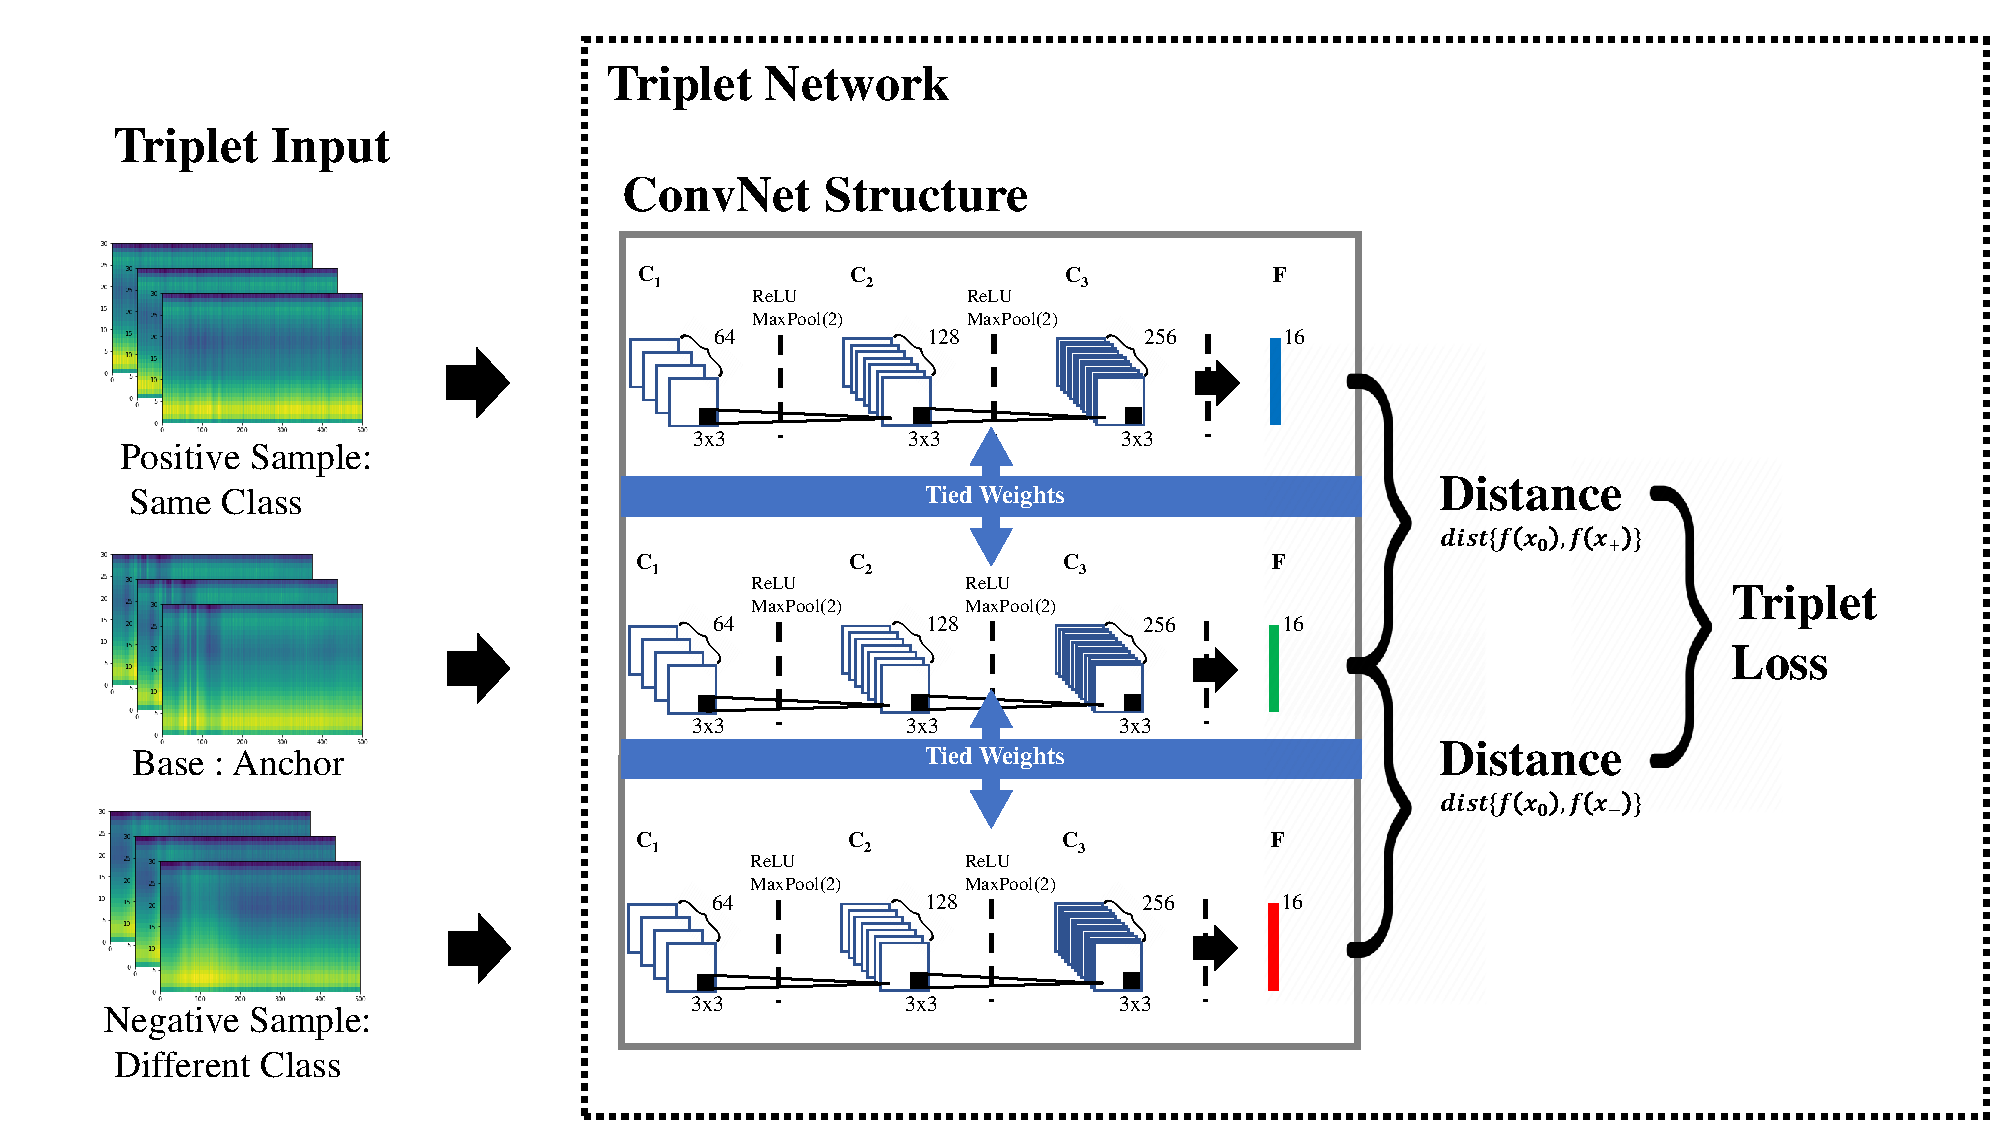
\includegraphics[width=\textwidth]
        {fig_convnet_v1.pdf}
    \caption{ConvNet structure.} \label{fig2}
\end{figure*}
% Structure
Our ConvNet model is consists of three filters and output fully-connected (FC) layer as seen in (item (b) in Fig.~\ref{fig1}). The depth of 3x3 sized ConvNet filters are empirically chosen as (64,128,256) with stride 1 and ReLU activation function. The size of FC layer is 16. Output FC layers are go through sigmoid activation function and normalized using $L2$ distance.
